\documentclass[conference]{IEEEtran}

\usepackage{amsmath}
\usepackage{graphics}
\usepackage{graphicx}

\bibliographystyle{/home/rsheissa/papers/icccas/ieeebib}

\begin{document}

% paper title
\title{A CAD Tool for Automated Design of Low-noise Nullor Based Amplifiers}

% author names and affiliations
\author{Arturo Sarmiento-Reyes, Roberto Casta\~neda-Sheissa, Luis Hern\'andez-Mart\'inez, H\'ector V\'azquez-Leal\\ National Institute for Astrophysics, Optics and Electronics\\
Electronics Department, CAD Group\\ P.O. Box 51, 72000, Puebla, Pue., Mexico}

% make the title area
\maketitle

\begin{abstract}
Low Noise Amplifers (LNA's) have become important for wideband-ultrawideband radio, microwave and cell-phone designers. In the design methodology, the LNA is composed by a nullor which represents an ideal active gain, i.e. the plant to be controlled by the feedback network which is usually constituted by passive components.\\
The paper shows that the noise calculation for these passive components and the synthesis of the first stage of the nullor can be automatically done. The automation is verified by means of a program that designs the feedback network and selects the right device to accomplish the noise specs provided by the designer.
\end{abstract}

\section{Introduction}
The low noise amplifier is a system where the noise level is carefully handled; it is usually the first block in a radio receiver that amplifies the signal from the antenna with as little distortion and additional noise as possible to be suitable for being processed by the first mixer \cite{svelto}.

The design of analogue electronic circuits has often been classified as an art under the assumption that no systematic procedures or methodologies have been developed. Experience has been the major way to produce knowledge regarding analogue design. The traditional way to obtain a new design is by carrying out some modifications on an already existing circuit until it fulfils some specific features. Nevertheless this way of design results very cryptic and difficult to handle for students and young designers.

Structured design has raised as an alternative to accomplish the analogue design task. It is based on the concept that the design must start from an ideal solution --- which obviously fulfils any set of specifications. The structured design is oriented to optimise aspects such as noise, distorion and bandwidth from a block point of view \cite{verhoeven,nordholt}. This approach lets the designer to focus on only one design aspect at a time \cite{stoffels}.

This work is focused on the first block to be designed which is the noise block. The noise stage is always the first to be designed because main noise contributions come from this block. If we consider the blocks of Figure \ref{figure1}; when a resistance is reflected from the output to the input of the first block, the resistance is diminished by a value equal to the square of the gain. Then if a resistance is reflected from the output circuit of the second block to the input of the first block, then the resistance is diminished by the product of the squares of the individual gains \cite{vergers}. Therefore, the equivalent noise resistance of the block combination is be given by
\begin{equation}
R_{eq_T}=R_{eq_1}+\frac{R_{eq_2}}{{A_1}^2}+...+\frac{R_{eq_n}}{({A_1}^2)...({A_n}^2)}
\end{equation} 

In fact, this means that the main noise contribution belongs to the first block of the design.

\begin{figure}
	\centering
	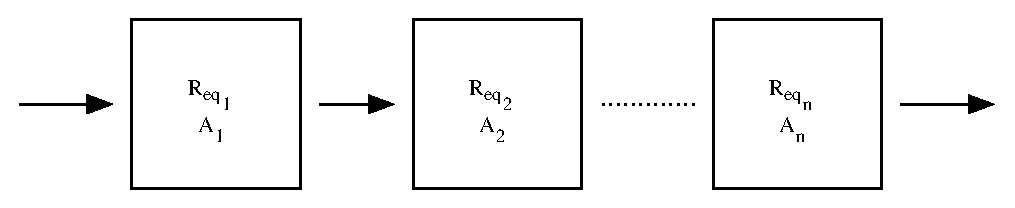
\includegraphics[scale=.55]{figures/amp_blocks.eps}
	\caption{Cascade of multiple stages.}
	\label{figure1}
\end{figure}


\section{Nullor-based amplifiers}
Within the structured design methodology, the nullor \-cons\-ti\-tu\-tes the active (ideal) block of the amplifier. The nullor is a two-port composed by two elements: {\bfseries \sffamily the nullator} connected at the input port and {\bfseries \sffamily the norator} connected at the output port. The transmission matrix of the nullor is given as \cite{carlin,moschytz}:
\begin{equation}\label{eq:abcd}
{K}
=
\left [ \begin{array}{cc}
\frac{1}{\mu}& \frac{1}{\gamma} \\\\
\frac{1}{\zeta}& \frac{1}{\beta}
\end{array}
\right ]
=
\left [ \begin{array}{cc}
0 & 0 \\ 0 & 0
\end{array}
\right ]
\end{equation}

It clearly results that the nullor possesses infinite gains for all four transfer relationships, voltage ($\mu$), current ($\alpha$), trans-conductance ($\gamma$) and trans-impedance ($\zeta$).

\begin{figure}[b]
	\centering
	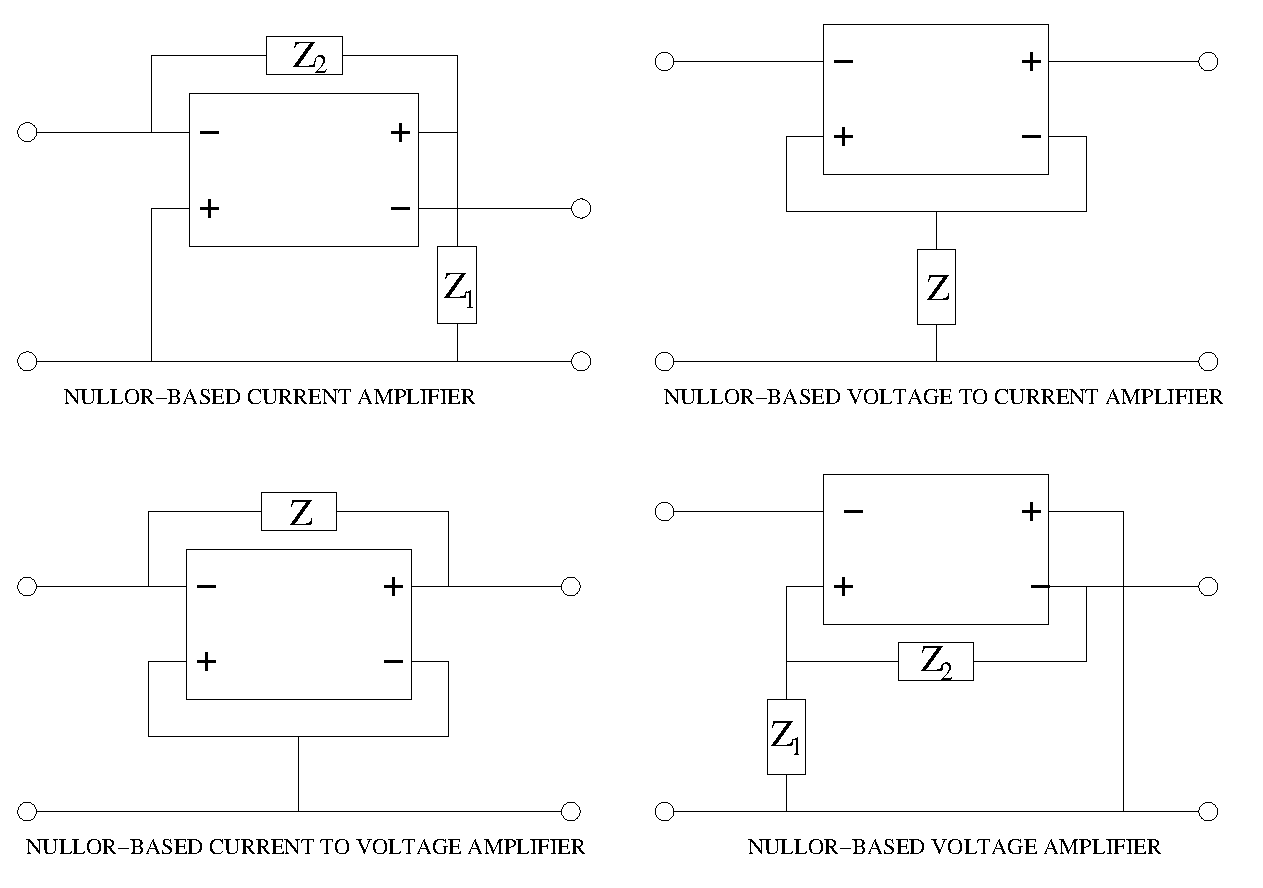
\includegraphics[scale=.4]{figures/nullor_based.eps}
	\caption{Negative-feedback Amplifiers.}
	\label{figure2}
\end{figure} 

\begin{figure}
	\centering
	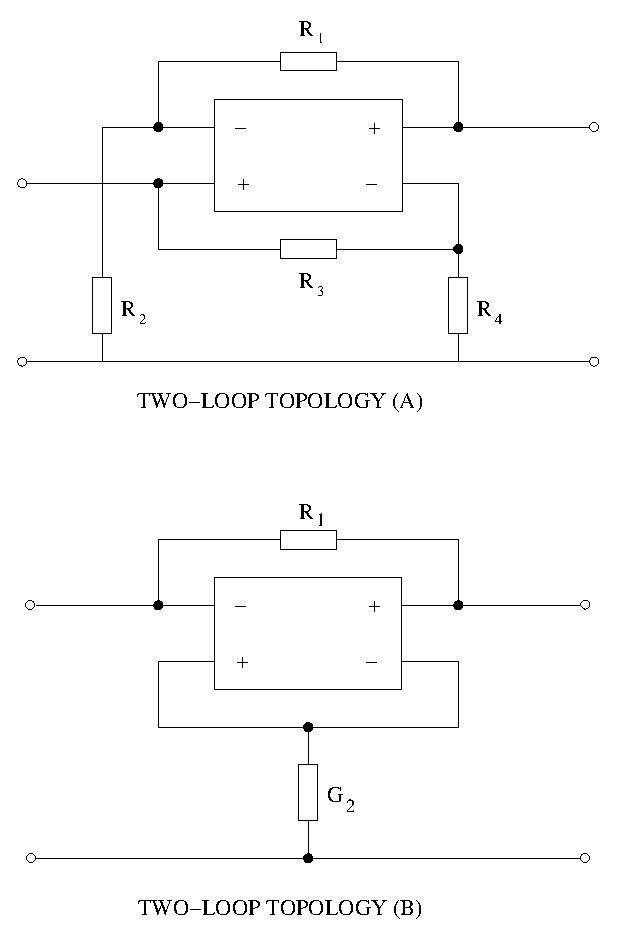
\includegraphics[scale=.55]{figures/basic_two_loops.eps}
	\caption{Two-loop Amplifiers.}
	\label{figure3}
\end{figure}

The basic one-loop amplifiers can be obtained when a passive feedback network is connected with the nullor as shown in Figure \ref{figure2}. If the one-loop amplifiers are combined then two basic two-loop types of amplifiers are generated as shown in Figure \ref{figure3}. The combination of voltage amplifier and current amplifier are referred as the {\bf two-loop topology (A)} and the combination of transconductance and transimpedance amplifiers are denoted as the {\bf two-loop topology (B)} \cite{nordholt,stoffels}.

Topology (B) can achieve all four kinds of transfers (voltage, current, transconductance and transimpedance), while Topology (A) can achieve all but the transconductance.

\subsection{Noise in the Amplifier}
In order to evaluate the noise in active devices the concept of noise factor is still widely used. The noise factor ({\it F}) is a quantity that compares the noise performance of a device against an ideal (noiseless) device. The noise power output of an ideal device is due to the thermal noise power of the source resistance \cite{ott}. Noise factor expressed in decibels is called noise figure ({\it NF}) and is expressed as:
\begin{equation}
NF=10log_{10}F
\end{equation}

Noise can be regarded in terms of power spectral densities originated from the passive network and the synthesised nullor. Because structured design uses power spectral densities for noise calculations then it is necessary to convert the noise figure term for the active devices into a noise voltage and current model, this method is explained in \cite{ott}.

A high-performance feedback amplifier accomplishes a specified transfer of a signal obtained from a signal source with known impedance to the load, while preserving the quality of the signal as much as possible. The feedback network affects the noise contribution of the noise sources present in the active circuit, usually increasing their contribution. The noise introduced by the transistor stages can be represented by a current and a voltage source placed at the input of the active part. 

The method to obtain the equivalent input noise sources for the single-loop topologies is detailed in \cite{sarmiento}, for the two-loop topologies a similar approach is used although it results rather cumbersome. The overall noise of the amplifier consists of two contributions. The first contribution comes from the feedback network, while the second contribution comes from the active devices.

Because the structured design constitutes in fact the \-sys\-te\-ma\-tic synthesis of the nullor with active devices (BJT or MOS transistors), noise design at the beginning of the process must perform a careful selection of the device which leads to an adequate calculation of bias value. 

MOSFET's are considered less suitable due to their large excess-noise contribution. For each transistor the voltage and current noise contributions are determined by the parameters and the bias current of the transistor \cite{stoffels}. The optimal first stage of the active circuit can be found by determining the optimal bias current. This is done by performing calculations that involve the internal parameters of the device ($g_m$, internal base resistance, collector resistance), the source signal (internal resistance) and the supply source.

An adequate bias value means that the noise contributed by the active device, the feedback-network and source complies at least to the noise limit established by the designer. 

\section{Program Structure}
A CAD tool --- {\bf NOMAD (Noise Optimisation in Modern Amplifier Design)} --- is aimed to simplify and automate the design process of negative-feedback amplifiers based on nullors. The designer provides a set of specifications such as amplifier transfer, configuration, gain, bandwidth and maximum allowed noise level among others.

\begin{figure}
	\centering
	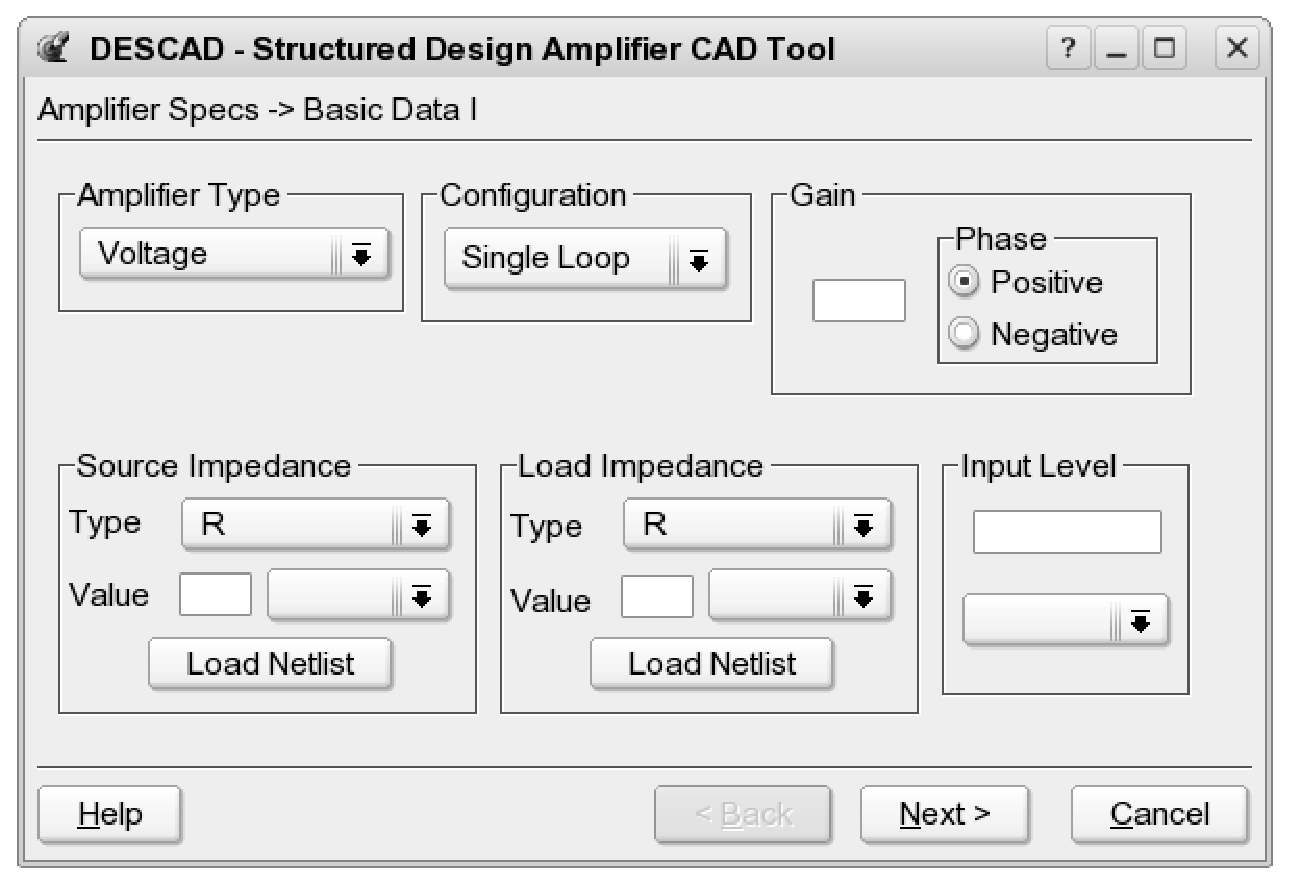
\includegraphics[scale=.4]{figures/descad_1.eps}
	\caption{Initial screen for NOMAD wizard.}
	\label{figure4}
\end{figure}

\begin{figure}
	\centering
	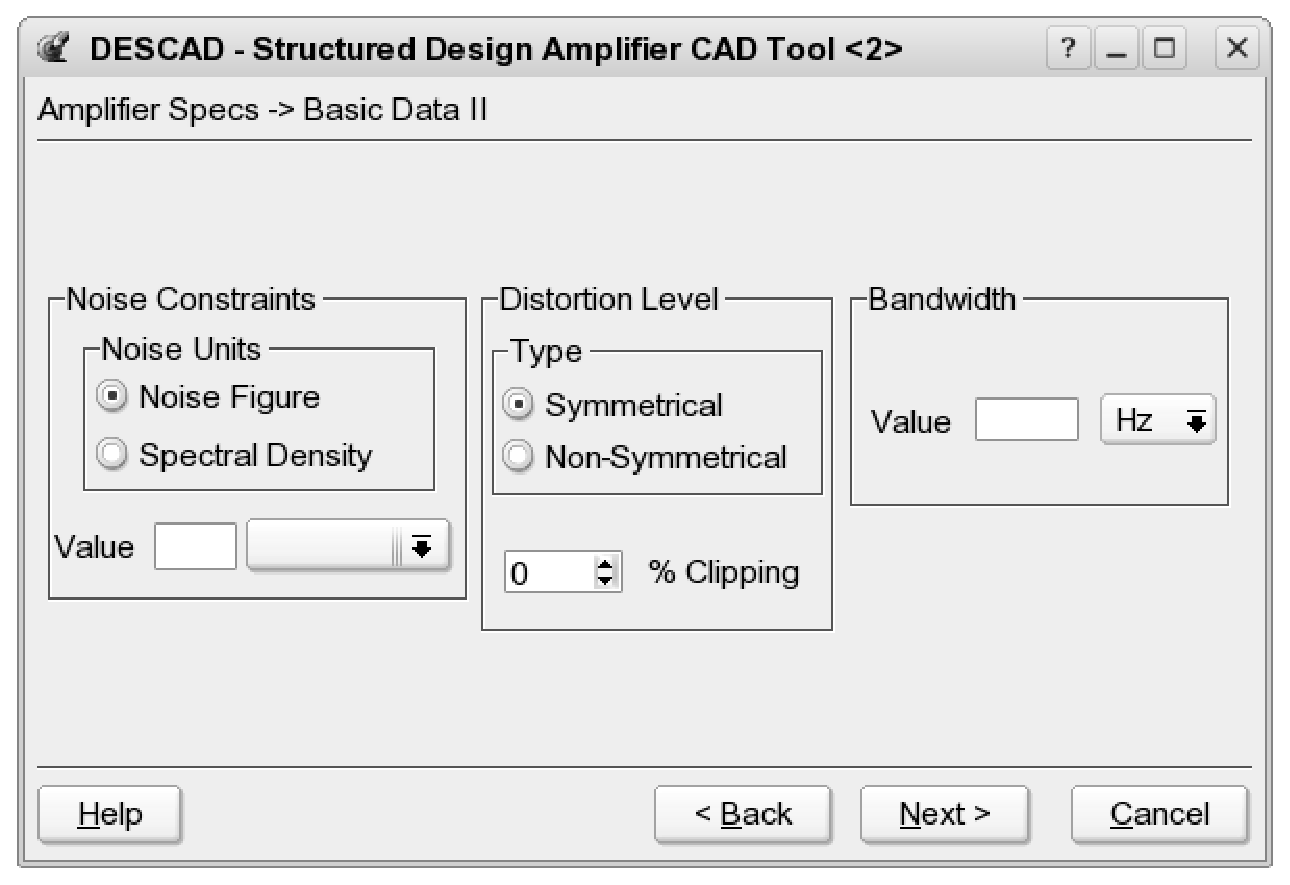
\includegraphics[scale=.4]{figures/descad_2.eps}
	\caption{Second window for NOMAD wizard.}
	\label{figure5}
\end{figure}

The tool has been developed in C++ for the backend, while the graphical user interface is programmed in Qt. The tool is aimed to run under Linux/Solaris without any constraints for special libraries. 

The main idea about the program is to guide the designer through the design process by means of a wizard approach. This wizard resorts to the use of windows as seen in Figure \ref{figure4}. The initial window is devoted to introduce the amplifier basic specs like the amplifier type, configuration, amplifier gain, source impedance, and load impedance.

The second window, Figure \ref{figure5}, expects three values to be specified: distortion,  bandwidth, and noise constraints. Noise value can be given in two different units. Noise figure value is given in decibel units while spectral density is given by $\frac{V}{\sqrt{Hz}}$ or $\frac{A}{\sqrt{Hz}}$.

Once the basic specs have been provided, the program performs the required calculations for the feedback network. This is displayed on a third window, entitled {\bf Noise, Step 1} (Figure \ref{figure6}). In order to accomplish the maximum allowed noise level it is necessary to have a trade-off between the noise contribution from the feedback network and the noise contribution from the active device that synthesizes the nullor. 

\begin{figure}
	\centering
	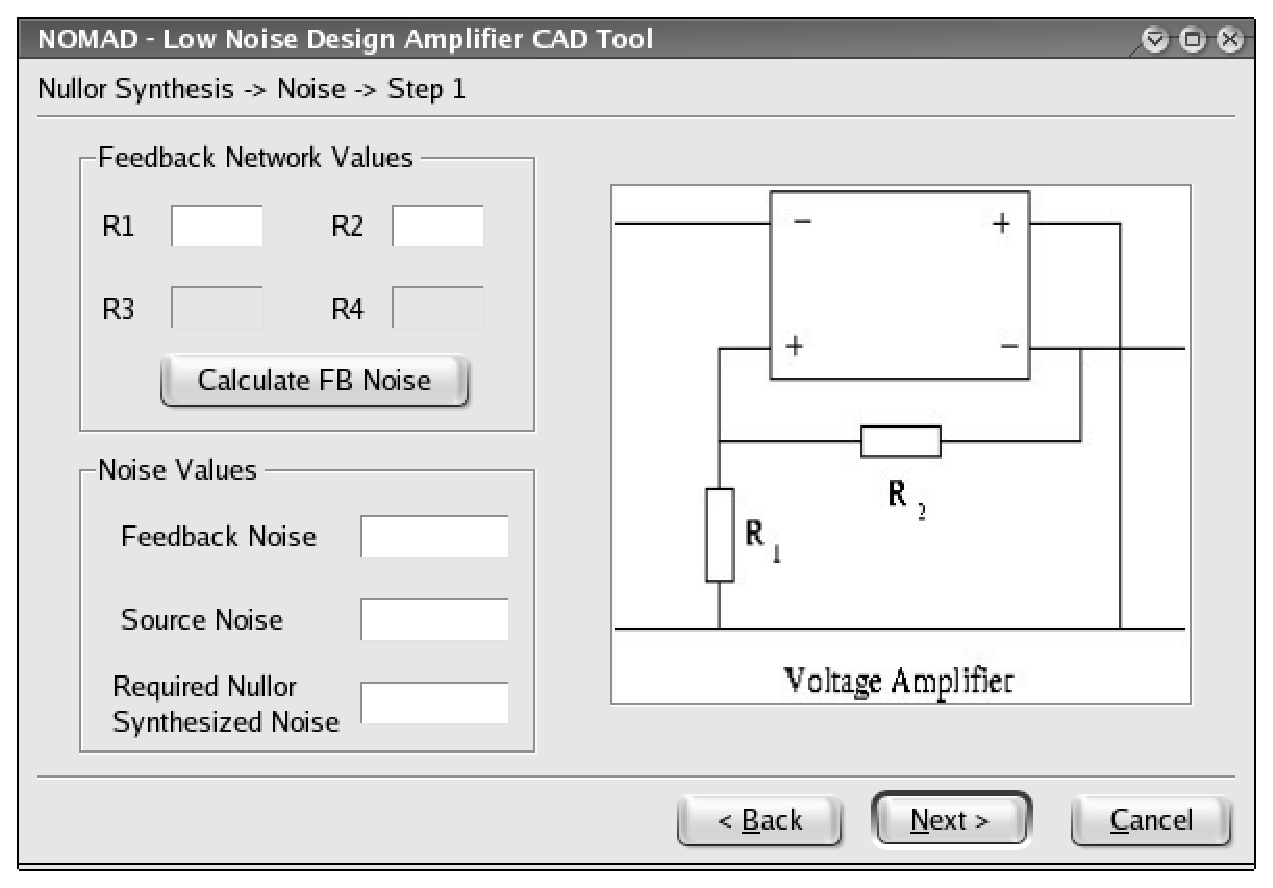
\includegraphics[scale=.4]{figures/descad_3.eps}
	\caption{Feedback noise calculation.}
	\label{figure6}
\end{figure}

\begin{figure}
	\centering
	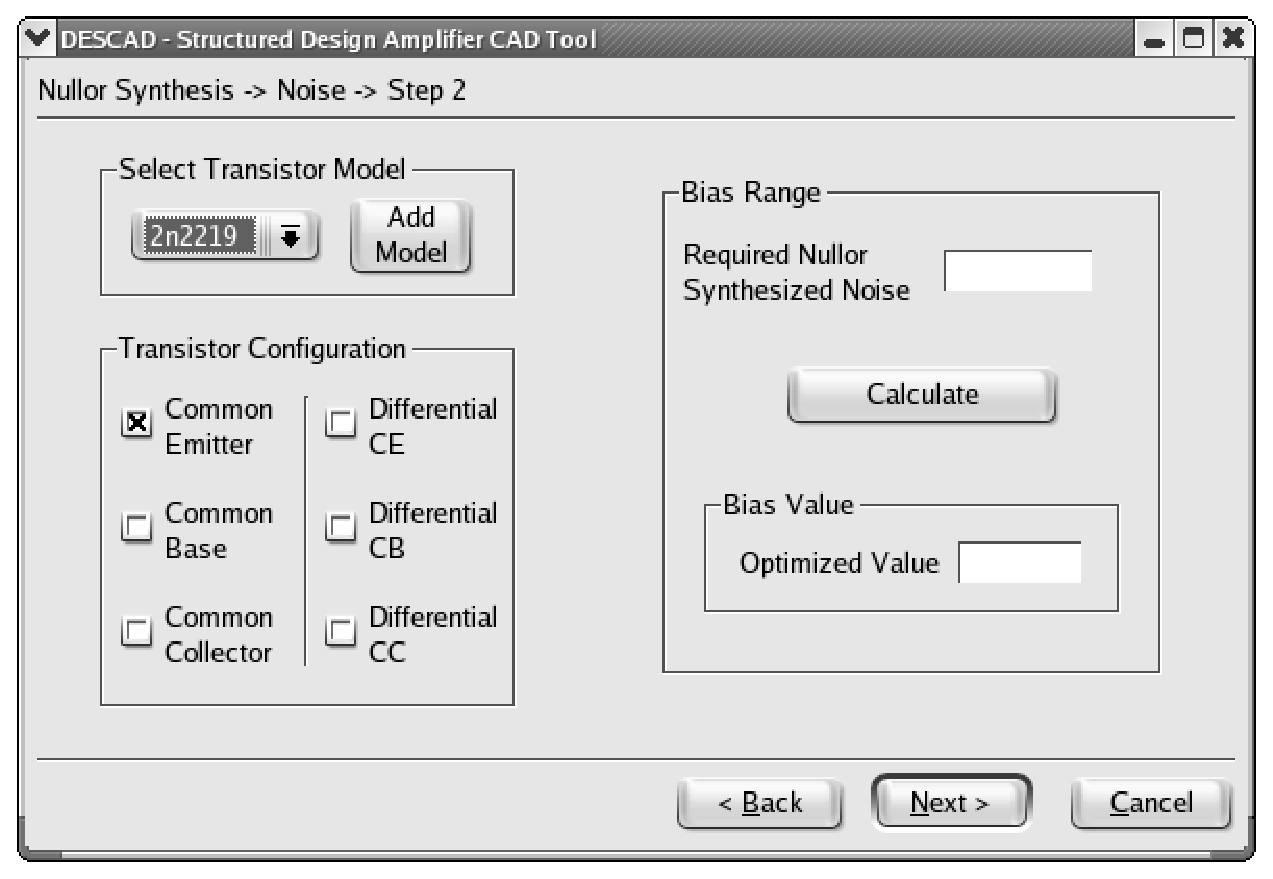
\includegraphics[scale=.4]{figures/descad_4.eps}
	\caption{Active device noise calculation.}
	\label{figure7}
\end{figure}

Figure \ref{figure7} shows the window entitled {\bf Noise, Step 2}. Here the designer can select between some transistor configurations (common emitter, common base, common collector, differential common emitter, differential common base, differential common collector). By clicking the {\bf Calculate} button a bias optimisation process is activated, and the value for optimum Ic is displayed. In case this process fails, a warning message is issued and the design process restarted from the first screen.

For the noise calculations on resistors and active devices SPICE-like calculations are performed \cite{spice}. The equations and the values obtained using them were validated after performing simulations on APLAC \cite{aplac} which includes a model that resembles the nullor behaviour. NOMAD finishes after delivering the final result for the amplifier, i.e. the value of the feedback resistors, the data regarding the active device parameters and the required bias current. 

\section{Example}
A design example is provided in order to show the function of the tool. The amplifier to be designed must fulfil these specs:

\begin{itemize}
\item Type = Voltage Amplifier
\item Configuration = Single Loop
\item Gain = 17 dB
\item Noise Figure = 2 dB
\item BW = 441 -- 451 MHz
\item Source Impedance= 100 $\Omega$
\end{itemize}

The calculated values for the feedback network are (Figure \ref{figure6}):
\begin{itemize}
\item R1 = 25 $\Omega$
\item R2 = 150 $\Omega$
\end{itemize}

Noise figure for the feedback network and source is 0.84 dB. Next step is to select the active device, configuration and then calculate the appropriate bias current.

The selected device is a BJT BFR520 \cite{bfr520} in common \-e\-mi\-tter configuration. This device has an excellent low-noise figure performance and is adequate for RF wideband applications. The selected bias current value is 3.4 mA. The noise figure for this bias value is 1.03dB. The total noise figure for the amplifier is 1.7 dB, this means that the tool can compute the adequate values for the resistors and bias value for the active device.

In order to verify if the design has fulfilled the specs, the resulting amplifier is simulated in APLAC. The schema is shown in Figure \ref{figure8}. The nullor is replaced by an ideal op-amp, though this element is not a nullor, its behaviour is the closest to it. Figure \ref{figure9} shows that the bias value for the BFR520 is the optimum to obtain the lowest noise figure. Figure \ref{figure10} shows the noise behaviour against frequency. As we can see this amplifier is within limits for a low-noise amplifier and accomplish the given specs.

\begin{figure}
	\centering
	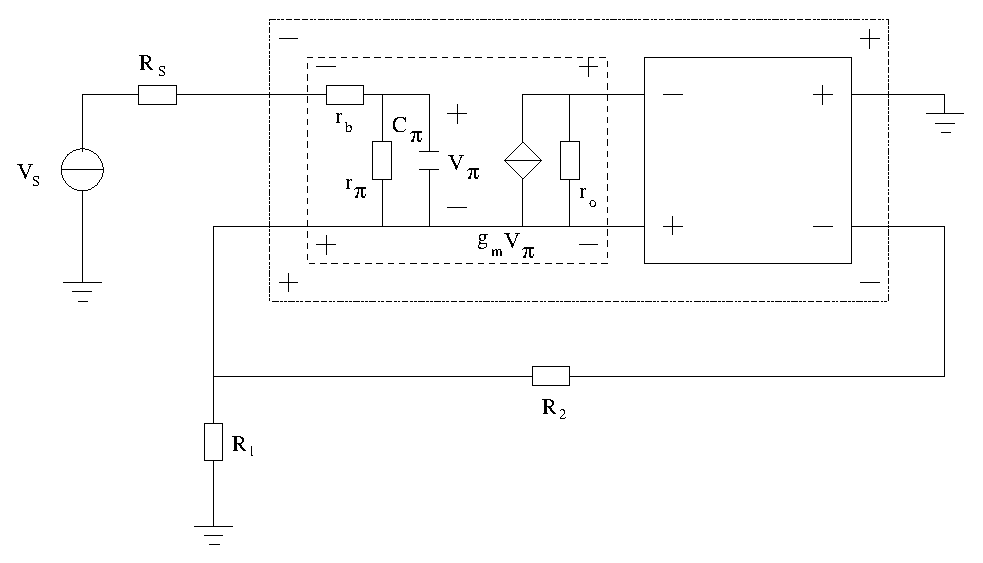
\includegraphics[scale=.4]{figures/amp_simulation.eps}
	\caption{Schema to simulate the nullor implementation.}
	\label{figure8}
\end{figure}

\begin{figure}
	\centering
	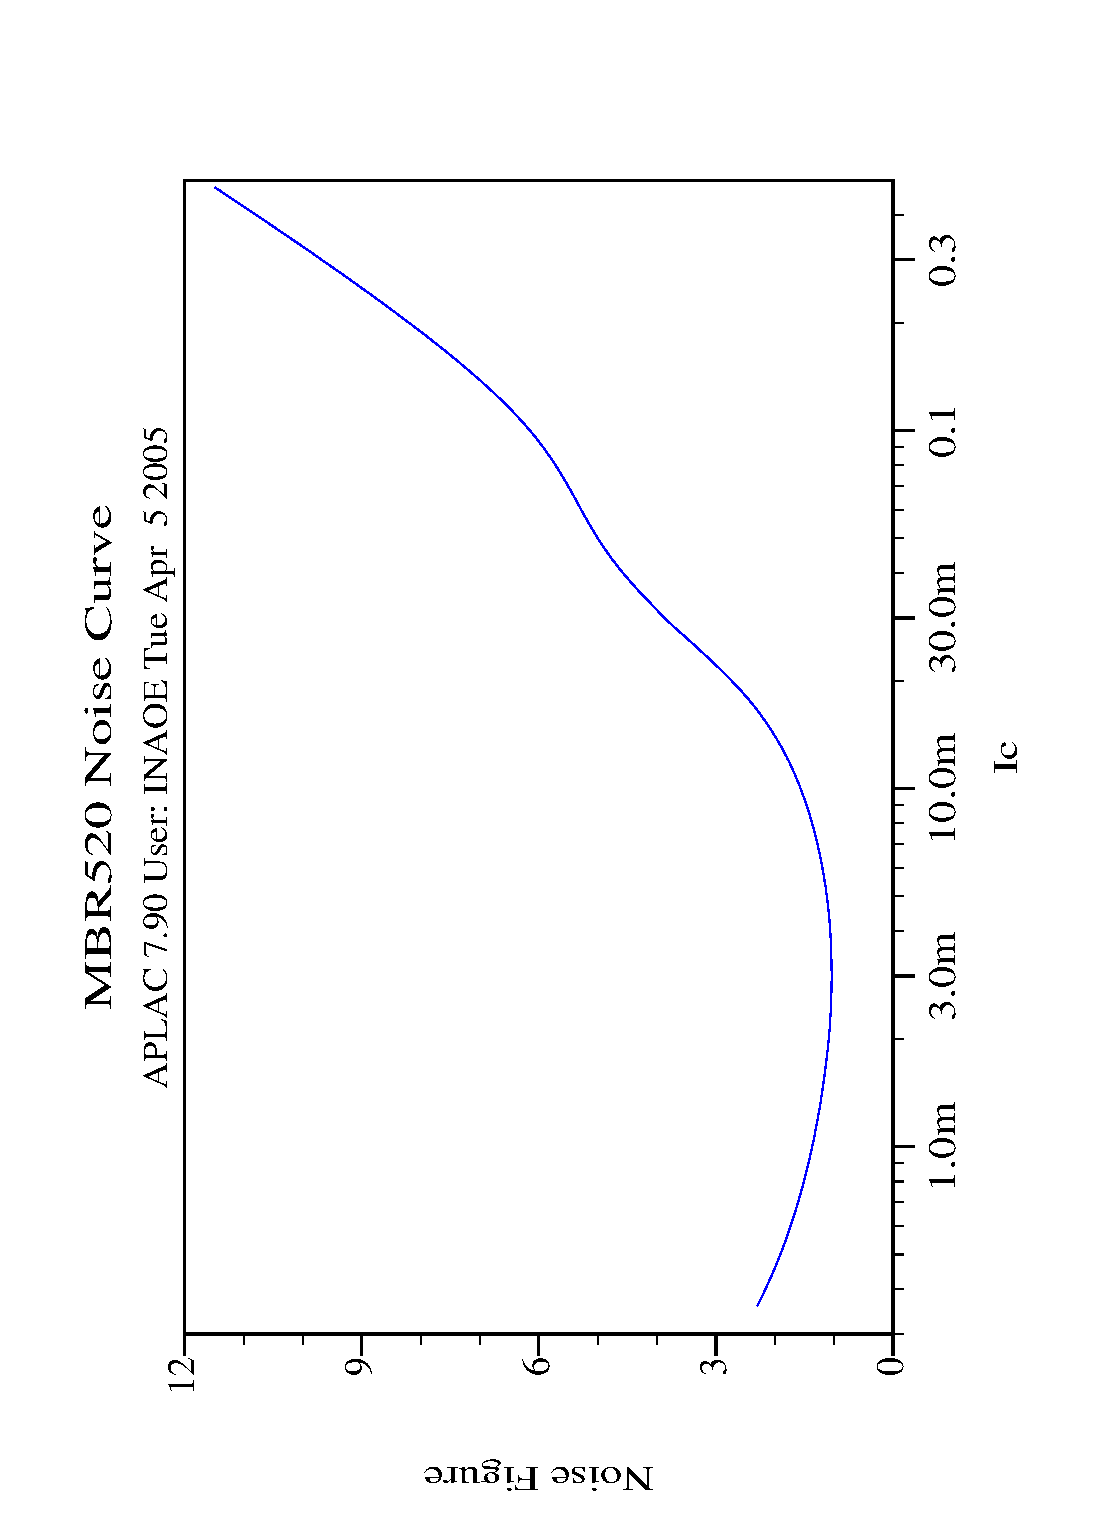
\includegraphics[scale=.35, angle=270]{figures/mbr520_noisecurves.eps}
	\caption{Noise figure versus collector current.}
	\label{figure9}
\end{figure}

\begin{figure}
	\centering
	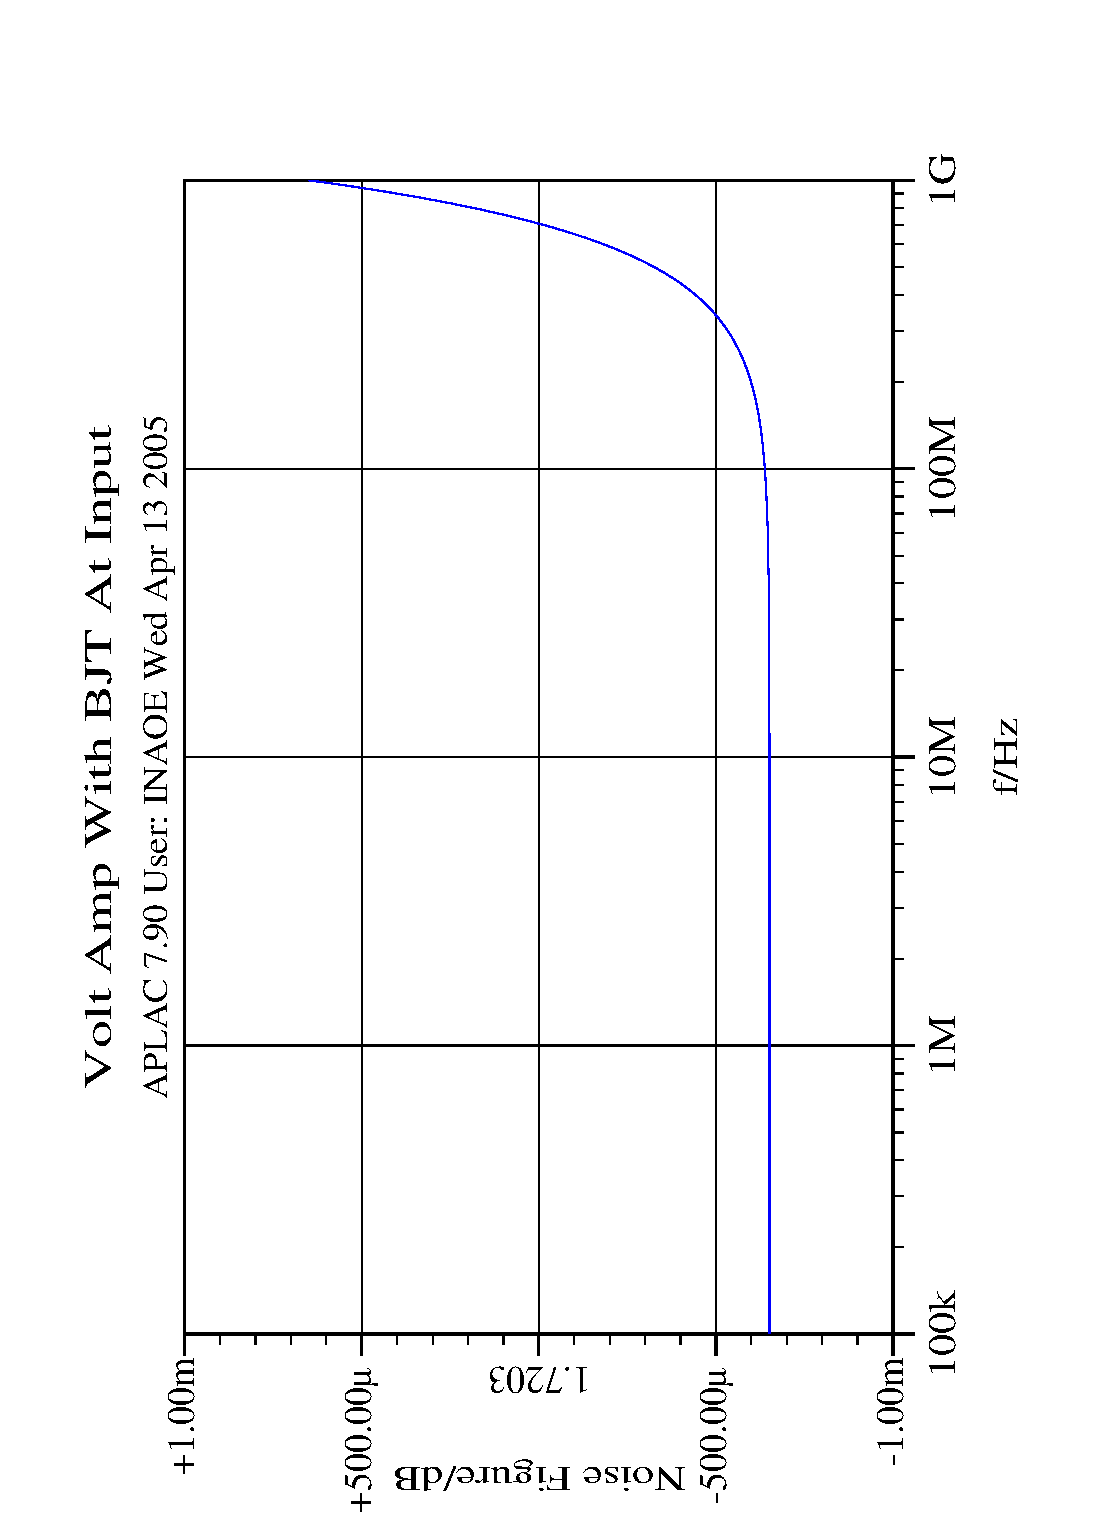
\includegraphics[scale=.35, angle=270]{figures/volt_amp_nf.eps}
	\caption{Frequency behaviour for voltage amplifier.}
	\label{figure10}
\end{figure}

\section{Conclusion}
It has been shown that it is possible to develop a CAD tool oriented to automate the design of low noise amplifiers based on a set of specifications provided by the designer. By means of a wizard approach the tool guides the designer in entering the amplifier specs in a step-by-step procedure. In case that the specs can not be fulfilled, the design process is stopped and taken to a previous step to modify one or more values. The development of the tool is based entirely on structured design, this shows that this design approach can speed up the design process obtaining accurate results.

\section*{Acknowledgement}
Roberto Casta\~neda Sheissa is holder of a scholarship from CONACyT M\'exico under contract 118652/120341. This work has been supported by a CONACyT M\'exico research project under grant 42588-Y.


\bibliography{bib/icccas}
\end{document}


